\documentclass[aspectratio=169,11pt]{beamer}

\usepackage{graphicx}
\usepackage{tikz}
\usetikzlibrary{positioning,arrows.meta}
\usepackage{xcolor}
\usepackage{booktabs}
\usepackage{tabularx}
\usepackage{array}
\usepackage{ragged2e}

\definecolor{GEUBlue}{RGB}{20,55,105}
\definecolor{GEULightBlue}{RGB}{238,244,251}
\definecolor{GEUGrey}{RGB}{90,90,90}
\definecolor{GEULightGrey}{RGB}{245,246,248}

\usetheme{default}
\setbeamertemplate{navigation symbols}{}
\setbeamertemplate{blocks}[rounded][shadow=false]
\setbeamercolor{normal text}{fg=black,bg=white}
\setbeamercolor{frametitle}{fg=GEUBlue}
\setbeamercolor{structure}{fg=GEUBlue}
\setbeamercolor{block title}{fg=GEUBlue,bg=GEULightBlue}
\setbeamercolor{block body}{fg=black,bg=GEULightBlue}
\setbeamerfont{frametitle}{size=\Large,series=\bfseries}

% Replace with the actual logo filename
\newcommand{\GEULogo}{graphicera_logo.png}

% Header and footer
\setbeamertemplate{headline}{%
  \begin{tikzpicture}[remember picture,overlay]
    \node[anchor=north east,xshift=-0.30cm,yshift=-0.12cm]
      at (current page.north east)
      {\includegraphics[height=0.62cm]{\GEULogo}};
  \end{tikzpicture}
  \vspace{0.72cm}
}
\setbeamertemplate{frametitle}{%
  \vspace{0.03cm}
  \insertframetitle\par
  \vspace{0.04cm}
  \textcolor{GEUBlue}{\rule{\textwidth}{0.9pt}}
  \vspace{0.03cm}
}
\setbeamertemplate{footline}{%
  \leavevmode
  \hbox{%
  \begin{beamercolorbox}[wd=.82\paperwidth,ht=0.32cm,dp=0.10cm,leftskip=.3cm]{author in head/foot}
    \tiny Department of Computer Science \& Engineering | Graphic Era (Deemed to be University)
  \end{beamercolorbox}%
  \begin{beamercolorbox}[wd=.18\paperwidth,ht=0.32cm,dp=0.10cm,rightskip=.3cm]{date in head/foot}
    \hfill\tiny\insertframenumber/\inserttotalframenumber
  \end{beamercolorbox}}
}

\newcommand{\smallnote}[1]{\vspace{0.08cm}{\scriptsize\color{GEUGrey}#1}}
\newcommand{\placeholder}[1]{\textit{\color{GEUGrey}#1}}

\title{\textbf{Project-Based Learning}\\[2mm]\large Phase-I Evaluation}
\author{\textbf{Vaultify -- A Secure Command-Line Password Manager in C++}\\Team ID: DSCPP-III-2026-T305}
\institute{Department of Computer Science \& Engineering\\Graphic Era (Deemed to be University), Dehradun}
\date{Academic Session 2026--27}

\begin{document}

% 1
\begin{frame}[plain]
\begin{tikzpicture}[remember picture,overlay]
\draw[GEUBlue,line width=3pt] (current page.north west) -- (current page.north east);
\node[anchor=north east,xshift=-0.45cm,yshift=-0.35cm] at (current page.north east)
{\includegraphics[height=1.0cm]{\GEULogo}};
\node[align=center,text width=.84\paperwidth] at ([yshift=-.15cm]current page.center)
{{\color{GEUBlue}\fontsize{22}{26}\selectfont\bfseries PROJECT-BASED LEARNING}\\[2mm]
 {\fontsize{15}{18}\selectfont PHASE-I EVALUATION}\\[5mm]
 {\color{GEUGrey}\large\bfseries Vaultify}\\[1mm]
 {\color{GEUGrey}\normalsize A Secure Command-Line Password Manager in C++}\\[3mm]
 {\color{GEUBlue}\normalsize Team ID: DSCPP-III-2026-T305}};
\node[align=center,anchor=south,yshift=.42cm] at (current page.south)
{\bfseries Department of Computer Science \& Engineering\\
Graphic Era (Deemed to be University), Dehradun\\[-1mm]
\scriptsize Academic Session 2026--27};
\end{tikzpicture}
\end{frame}

% 2
\begin{frame}{Team \& Mentor Details}
\begin{columns}[T,totalwidth=\textwidth]
\column{.48\textwidth}
\begin{block}{Team Information}
\begin{tabular}{@{}ll@{}}
\textbf{Team ID:} & DSCPP-III-2026-T305\\
\textbf{Semester:} & 3rd\\
\textbf{Section:} & B / ML2 / ML3\\
\textbf{Domain:} & Systems Programming\\ & / Utility Tools
\end{tabular}
\end{block}
\column{.48\textwidth}
\begin{block}{Team Members}
1.\quad Ashraya Mishra (Lead) -- 2510010429\\
2.\quad Udit Joshi -- 2510370397\\
3.\quad Yuvraj Singh -- 2510010591
\end{block}
\end{columns}
\vspace{2mm}
\begin{block}{Mentor}
Dr. Prabhdeep Singh
\hfill
\textbf{Interactions completed:} \underline{\hspace{4mm}2\hspace{4mm}}
\end{block}
\end{frame}

% 3
\begin{frame}{Problem Statement \& Motivation}
\begin{block}{Problem Statement}
\small Most users maintain accounts on dozens of platforms but can only reliably remember a handful of passwords -- leading to reuse and weak passwords that expose accounts to credential-stuffing after any single breach.
\end{block}
\vspace{1mm}
\begin{columns}[T,totalwidth=\textwidth]
\column{.48\textwidth}
\textbf{\color{GEUBlue}Motivation}
\begin{itemize}\itemsep1pt\small
\item Password reuse is widespread and risky
\item One breach can compromise many accounts
\item Existing tools are closed or paid
\end{itemize}
\column{.48\textwidth}
\textbf{\color{GEUBlue}Target Users / Stakeholders}
\begin{itemize}\itemsep1pt\small
\item Individuals managing many accounts
\item Students wanting a transparent tool
\item Users seeking a local alternative
\end{itemize}
\end{columns}
\end{frame}

% 4
\begin{frame}{Objectives}
\textbf{\color{GEUBlue}Project Objectives}
\vspace{2mm}
\begin{enumerate}\itemsep5pt
\item Build a secure, functional command-line password manager in C++.
\item Implement a hash table-based vault for O(1) credential storage and retrieval.
\item Apply symmetric encryption and hash-based master password verification.
\item Ensure persistence of vault data across sessions using file handling.
\item Demonstrate practical, real-world application of core DS and OOP concepts.
\end{enumerate}
\vfill
\begin{center}
\colorbox{GEULightBlue}{\parbox{.80\textwidth}{\centering
\textbf{Key Objective:} Deliver a working, cross-platform CLI password manager that securely stores and retrieves credentials without ever storing the master password in plain text.}}
\end{center}
\end{frame}

% 5
\begin{frame}{Proposed Solution}
\begin{columns}[T,totalwidth=\textwidth]
\column{.48\textwidth}
\textbf{\color{GEUBlue}Proposed Approach}
\begin{enumerate}\itemsep3pt
\item Entry -- credential data class
\item Vault -- hash table storage layer
\item Crypto -- encryption \& hashing logic
\item FileHandler -- persistent storage
\item CLI -- menu-driven user interface
\end{enumerate}
\column{.48\textwidth}
\textbf{\color{GEUBlue}Key Features}
\begin{itemize}\itemsep2pt\small
\item Add / retrieve / update / delete / list
\item Master password auth via hash verification
\item Symmetric encryption of stored passwords
\item Persistent, file-based vault storage
\item Cross-platform (Windows \& Linux)
\end{itemize}
\end{columns}
\vfill
\smallnote{The hash table gives O(1) average lookup by site; encryption and hashed authentication ensure no credential is ever stored in plain text.}
\end{frame}

% 6
\begin{frame}{Integration of PBL Course Concepts}
\scriptsize
\begin{center}
\renewcommand{\arraystretch}{1.25}
\begin{tabularx}{.96\textwidth}{@{}>{\bfseries}p{3.0cm}X p{2.5cm}@{}}
\toprule
Course & Concepts Applied & Project Module\\
\midrule
Data Structures in C & Hash Tables, Hash Functions \& Collision Resolution, Stacks, File Structures & Vault, Recently-Accessed Stack\\
OOPs with C++ & Classes \& Encapsulation, Constructors, File Handling, Exception Handling & Entry, Crypto, FileHandler, CLI\\
\bottomrule
\end{tabularx}
\end{center}
\vfill
\begin{center}
\colorbox{GEULightBlue}{\parbox{.86\textwidth}{\centering
\textbf{Requirement:} Demonstrate meaningful integration of both subjects in \textbf{one} project.}}
\end{center}
\end{frame}

% 7
\begin{frame}{System Architecture / Workflow}
\begin{center}
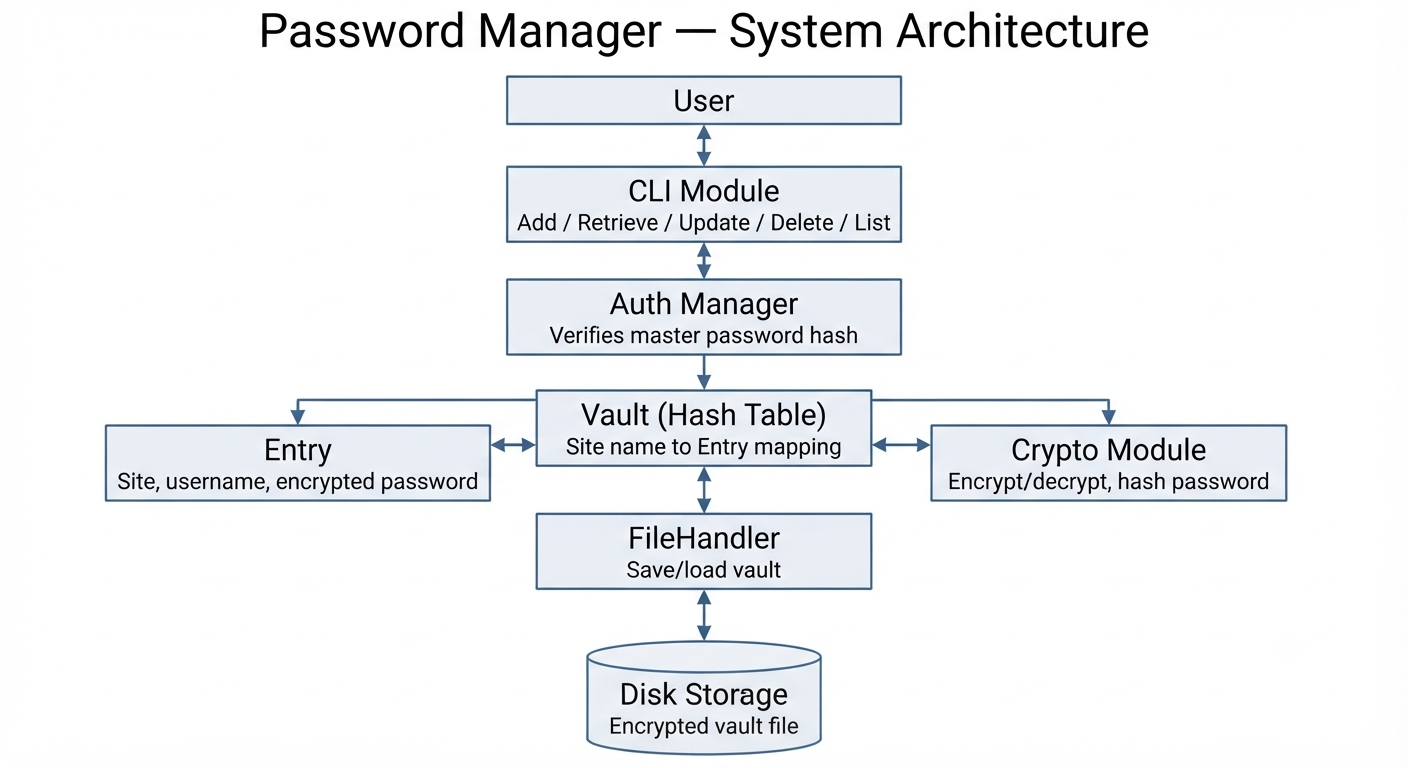
\includegraphics[width=0.85\linewidth,height=5.6cm,keepaspectratio]{architecture.png}
\end{center}
\vspace{3mm}
\begin{columns}[T,totalwidth=\textwidth]
\column{.48\textwidth}
\textbf{\color{GEUBlue}Major Components}
\begin{itemize}\itemsep2pt
\item CLI Module \& Auth Manager
\item Vault (Hash Table) \& Entry
\item Crypto Module \& FileHandler
\end{itemize}
\column{.48\textwidth}
\textbf{\color{GEUBlue}Data / Control Flow}
\begin{itemize}\itemsep2pt
\item User request flows through CLI to the Vault
\item Vault encrypts/decrypts via Crypto, persists via FileHandler
\item FileHandler reads/writes the encrypted vault file on disk
\end{itemize}
\end{columns}
\end{frame}

% 8
\begin{frame}{Technology Stack \& Methodology}
\begin{columns}[T,totalwidth=\textwidth]
\column{.48\textwidth}
\begin{block}{Technology Stack}
\begin{itemize}\itemsep2pt
\item Programming: C++
\item Storage: Local encrypted flat file
\item Tools / Framework: Standard C++ (no external libraries)
\item IDE: Visual Studio Code
\item Version Control: Git
\end{itemize}
\end{block}
\column{.48\textwidth}
\begin{block}{Development Methodology}
\begin{enumerate}\itemsep2pt
\item Requirement Analysis
\item System Design
\item Implementation
\item Testing
\item Evaluation
\end{enumerate}
\end{block}
\end{columns}
\vfill
\begin{center}
\smallnote{C++ was chosen to directly apply DS and OOP concepts from the course; a local encrypted file avoids external dependencies, keeping the tool lightweight and fully self-contained.}
\end{center}
\end{frame}

% 9
\begin{frame}{Initial Progress \& Team Contribution}
\begin{columns}[T,totalwidth=\textwidth]
\column{.44\textwidth}
\textbf{\color{GEUBlue}Progress Achieved}
\begin{itemize}\itemsep3pt
\item Problem study \& existing-solution analysis completed
\item Requirements and core goals finalized
\item System architecture designed
\item Core class structure (Entry, Vault, Crypto) scoped
\item Development environment \& toolchain set up
\end{itemize}
\column{.52\textwidth}
\textbf{\color{GEUBlue}Individual Contribution}
\vspace{2mm}
\scriptsize
\begin{tabularx}{\textwidth}{@{}p{2.3cm}p{2.0cm}X@{}}
\toprule
Member & Role & Contribution\\
\midrule
Ashraya Mishra & Lead/Developer & Vault module, FileHandler, system integration\\
Udit Joshi & Developer & Entry class, Crypto module (encryption \& hashing)\\
Yuvraj Singh & Developer & CLI module, output formatting, cross-platform testing\\
\bottomrule
\end{tabularx}
\end{columns}
\end{frame}

% 10
\begin{frame}{Roadmap, Expected Outcomes \& References}
\begin{columns}[T,totalwidth=\textwidth]
\column{.47\textwidth}
\textbf{\color{GEUBlue}Roadmap}
\begin{enumerate}\itemsep3pt
\item Phase-I: Proposal \& Design
\item Phase-II: Development
\item Phase-III: Final Implementation
\end{enumerate}
\vspace{2mm}
\textbf{\color{GEUBlue}Expected Outcomes}
\begin{itemize}\itemsep2pt
\item Fully working, cross-platform CLI manager
\item Secure, encrypted local credential storage
\item Clean, reusable C++ source code
\end{itemize}
\column{.47\textwidth}
\textbf{\color{GEUBlue}References}
\begin{enumerate}\itemsep2pt
\item Thareja, R. -- \textit{Data Structures Using C++}
\item cppreference.com -- C++ \& STL reference
\item GeeksforGeeks -- hashing, file handling
\item OWASP Foundation -- Password Storage Cheat Sheet
\end{enumerate}
\vfill
\begin{center}
\colorbox{GEUBlue}{\parbox{.78\textwidth}{\centering\color{white}\textbf{Thank You}\\Questions \& Suggestions}}
\end{center}
\end{columns}
\end{frame}

\end{document}